\section{Оценка аппаратной сложности и масштабируемости вычислительного ядра}

В данном разделе приводится детальный анализ низкоуровневых характеристик разработанного ядра, включая аппаратную сложность приоритетных очередей, многопоточную масштабируемость и накладные расходы очередей обмена сообщениями.
Встроенные счетчики процессора регистрируют количество тактов на операции вставки и извлечения в однопоточном режиме для алгоритма ALT. Таблица \ref{tab:hardware_queues} и рисунок \ref{fig:push_pop_cycles_comparison} содержат результаты этих измерений.

\begin{table}[htbp]
\centering
\small
\renewcommand{\arraystretch}{1.2}
\caption{Аппаратная сложность и накладные расходы операций с очередями приоритетов в алгоритме ALT}
\label{tab:hardware_queues}
\begin{tabularx}{\linewidth}{|L|Y|Y|Y|}
\hline
\textbf{Тип очереди приоритетов} & \textbf{Такты на вставку} & \textbf{Такты на извлечение} & \textbf{Средняя доля накладных расходов (\%)} \\ \hline
Двоичная куча (2-ary) & $80{,}65$ & $186{,}62$ & $50{,}15\%$ \\ \hline
$4$-арная куча & $77{,}01$ & $166{,}66$ & $50{,}95\%$ \\ \hline
$8$-арная SoA-куча & $75{,}58$ & $174{,}09$ & $49{,}88\%$ \\ \hline
$16$-арная куча & $75{,}06$ & $178{,}25$ & $50{,}97\%$ \\ \hline
Корзиночная очередь & $74{,}61$ & $77{,}85$ & $43{,}34\%$ \\ \hline
Поразрядная очередь & $82{,}53$ & $107{,}88$ & $48{,}13\%$ \\ \hline
Векторизованная дельта-очередь & $74{,}73$ & $77{,}76$ & $43{,}17\%$ \\ \hline
\end{tabularx}
\end{table}

\begin{figure}[htbp]
    \centering
    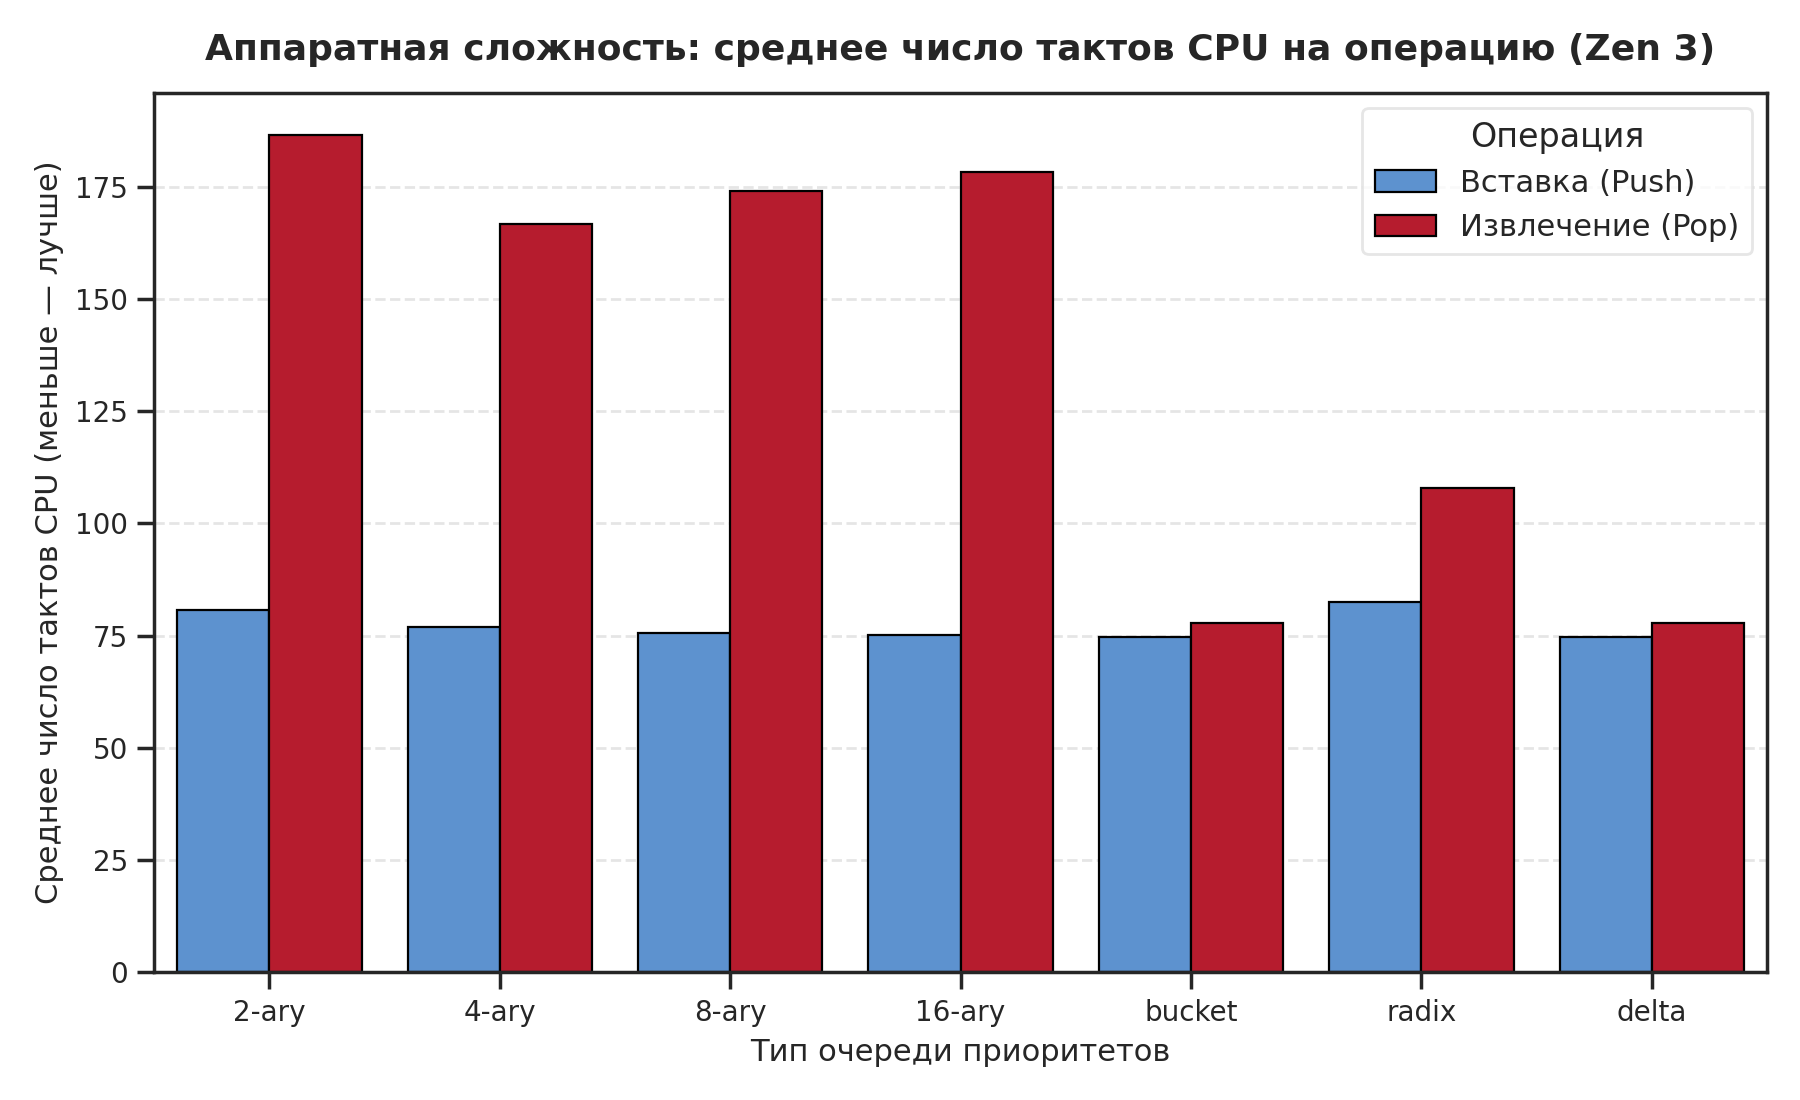
\includegraphics[width=0.85\linewidth,height=0.35\textheight,keepaspectratio]{assets/images/push_pop_cycles_comparison.png}
    \caption{Аппаратная сложность: среднее число тактов процессора на операции вставки и извлечения в алгоритме ALT}
    \label{fig:push_pop_cycles_comparison}
\end{figure}

Для обеспечения сквозной прозрачности и верифицируемости экспериментальных графиков ниже приведено точное соответствие условных обозначений в легендах разработанным классам вычислительного ядра:
\begin{itemize}
    \item \texttt{2-ary}~-- классическая двоичная куча на базе непрерывного вектора (\texttt{Strict2AryHeap});
    \item \texttt{4-ary}~-- векторизованная $4$-арная куча с AVX2-оптимизацией раскрытия потомков (\texttt{Strict4AryHeap});
    \item \texttt{8-ary}~-- $8$-арная SoA-куча (структура массивов) с отложенной (ленивой) реструктуризацией (\texttt{Strict8ArySoALazyHeap}), показавшая наилучшую сбалансированность;
    \item \texttt{16-ary}~-- $16$-арная куча с высокой степенью ветвления (\texttt{Strict16AryHeap});
    \item \texttt{delta}~-- векторизованная приближенная дельта-очередь с шагом $\Delta = 16$ и быстрым branchless-поиском (\texttt{DeltaQueue});
    \item \texttt{bucket}~-- приближенная корзиночная очередь с размером ведра $\Delta = 16$ на базе связанных списков (\texttt{DeltaBucketQueue});
    \item \texttt{radix}~-- потокобезопасная поразрядная куча со скользящими интервалами весов (\texttt{SafeRadixHeap}).
\end{itemize}

Векторизованная $8$-арная SoA-куча (\texttt{Strict8ArySoAHeap}) превосходит стандартную двоичную кучу по скорости вставки элемента на $6{,}28\%$ ($75{,}58$~такта против $80{,}65$~такта), а по извлечению элемента~-- на $6{,}71\%$ ($174{,}09$~такта против $186{,}62$~такта), сохраняя стоимость на сверхвысоком уровне. При этом $4$-арная куча благодаря меньшей высоте дерева обходит двоичную по извлечению на $10{,}69\%$ ($166{,}66$~такта). Это подтверждает высокую эффективность применения структуры SoA (структура массивов) и AVX2 векторизации при поиске минимального потомка, который выполняется параллельно без ветвлений конвейера. Корзиночные структуры и DeltaQueue демонстрируют минимальное время операции извлечения (до $77{,}76$~тактов) благодаря обратно-логарифмической или отсутствующей зависимости от размера очереди.

Динамика изменения накладных расходов в зависимости от длины пути приведена на рисунке \ref{fig:queue_overhead_trend}.

\begin{figure}[htbp]
    \centering
    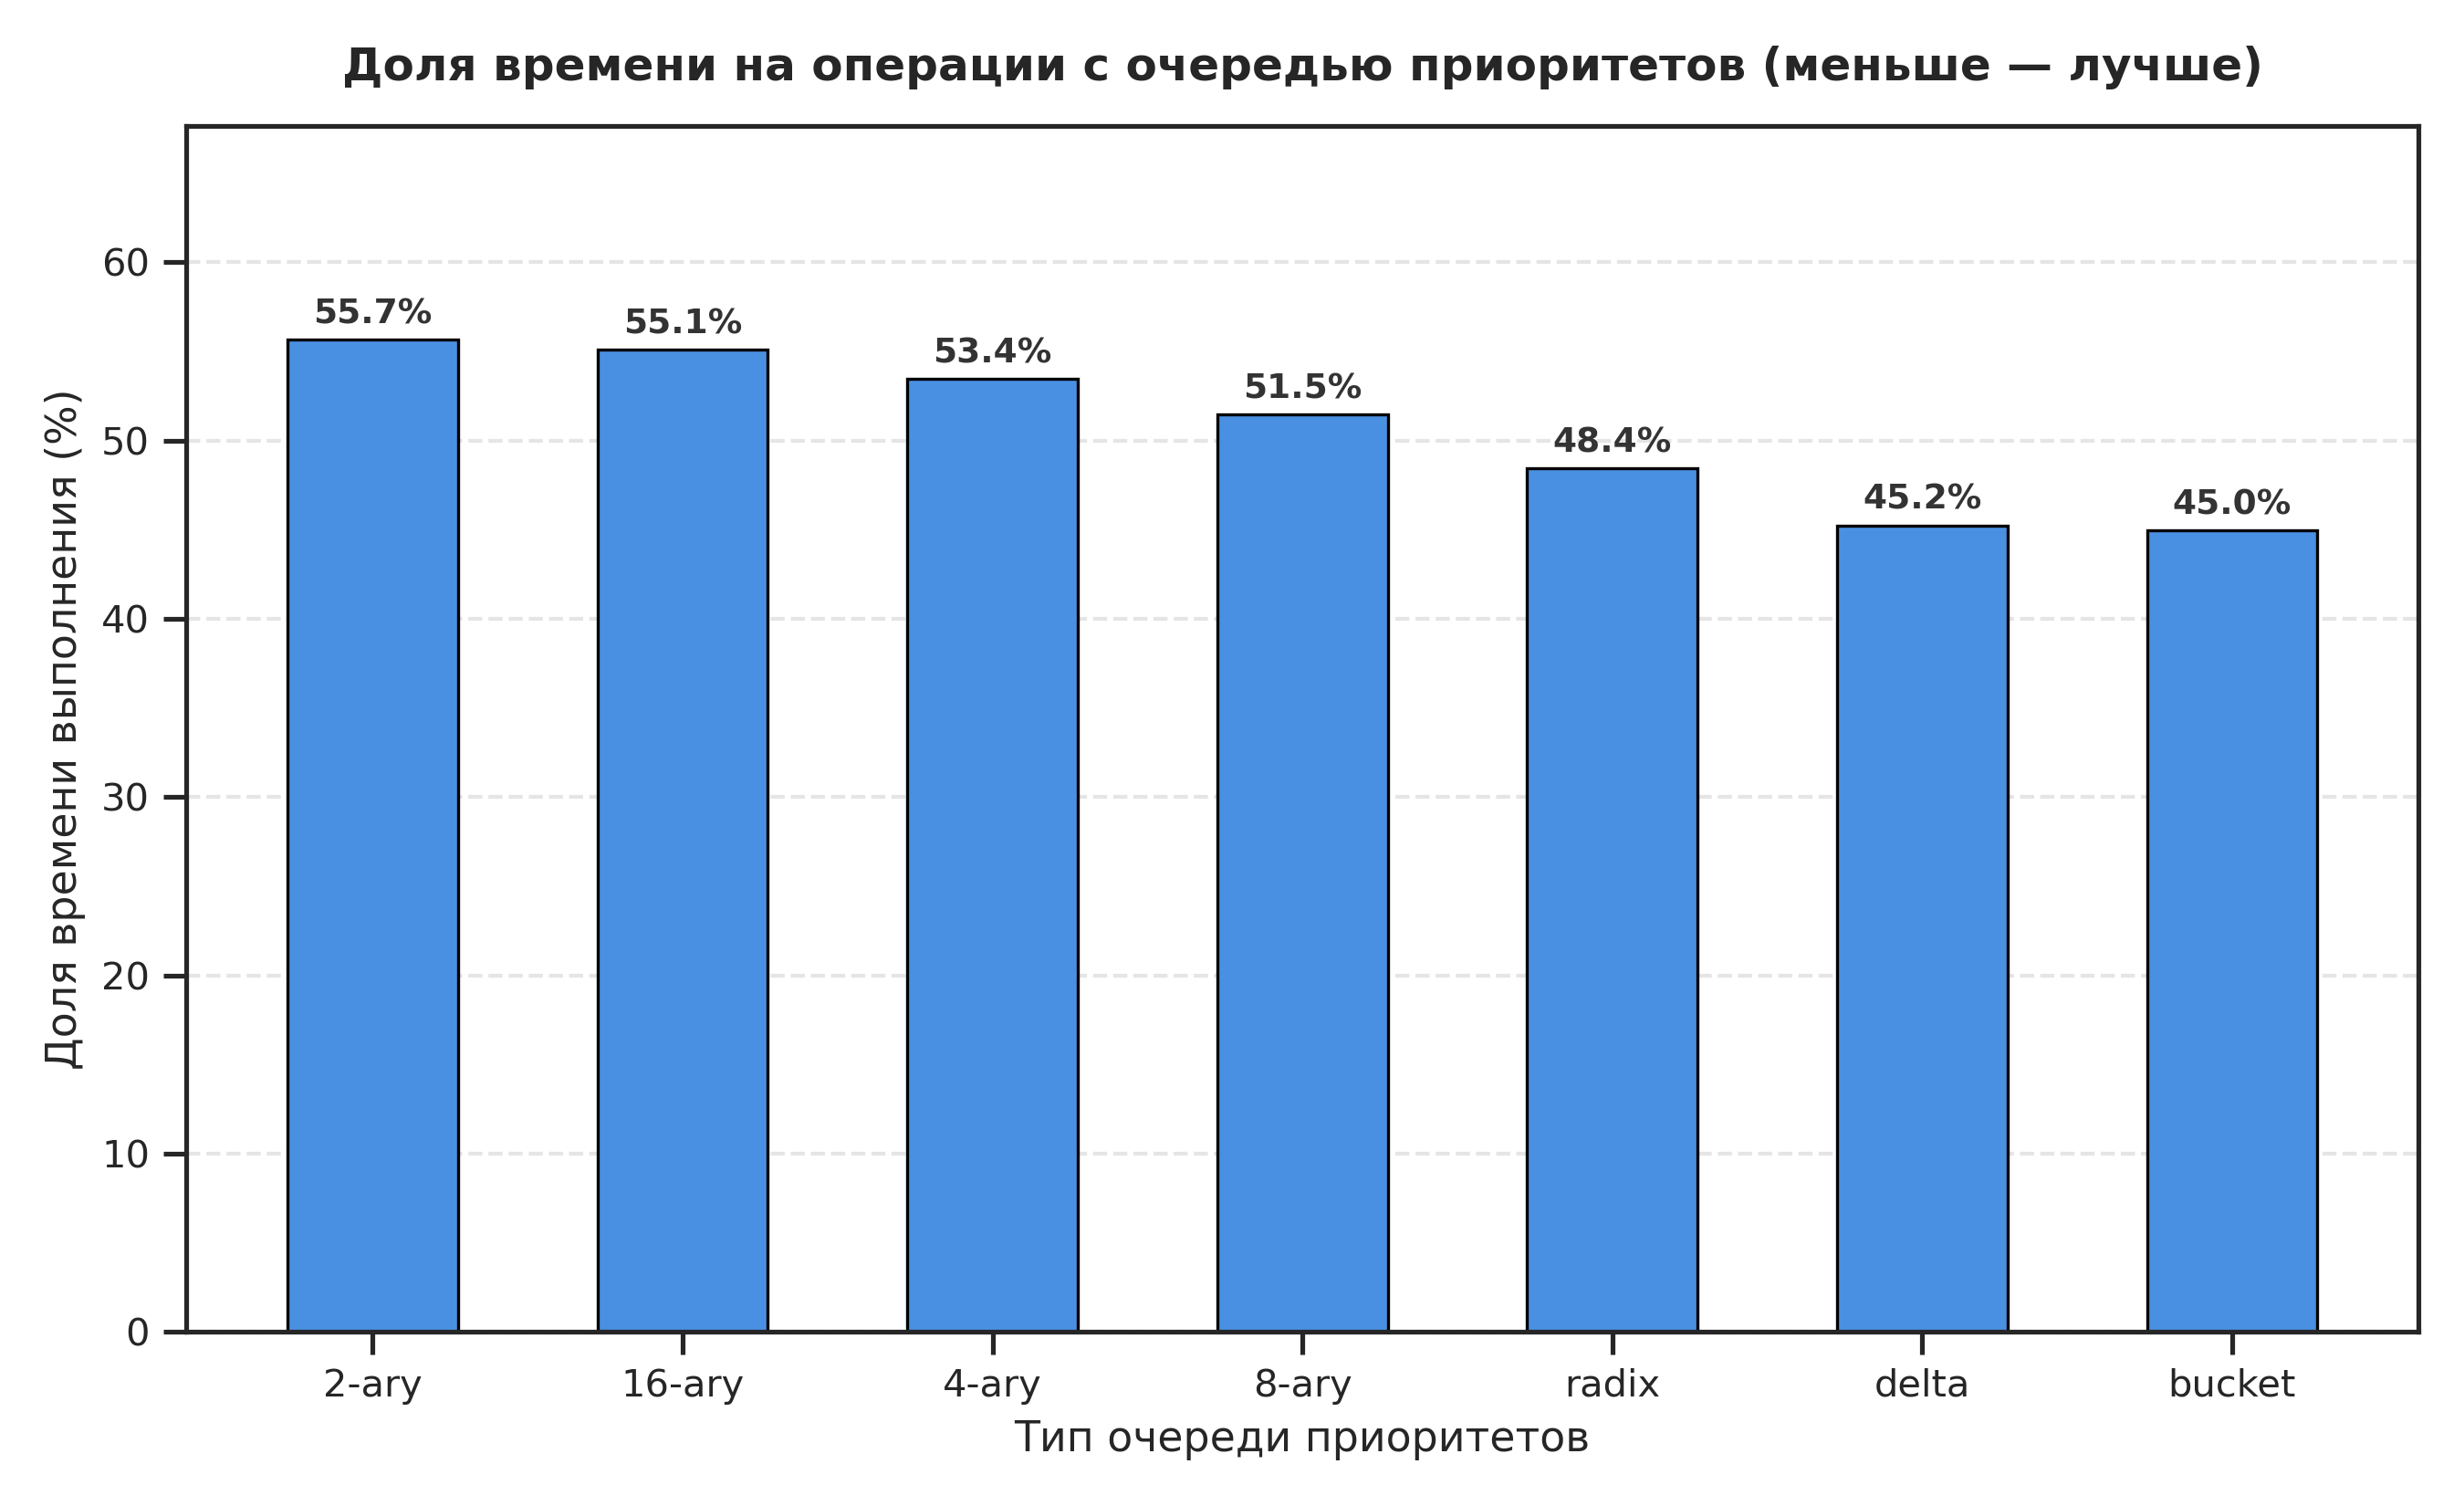
\includegraphics[width=0.85\linewidth,height=0.35\textheight,keepaspectratio]{assets/images/queue_overhead_trend.png}
    \caption{Накладные расходы очередей приоритетов в процентах от общего времени поиска пути с $95\%$-м доверительным интервалом}
    \label{fig:queue_overhead_trend}
\end{figure}

Анализ показывает, что доля времени, затрачиваемая на очереди приоритетов, варьируется от $48{,}08\%$ для высоконаправленного алгоритма ALT до $60{,}12\%$ для классического алгоритма Дейкстры (из-за огромного размера дерева поиска). DeltaQueue стабильно удерживает накладные расходы на самом низком уровне среди всех исследованных структур.

Для исследования масштабируемости программа измеряет пропускную способность на процессоре AMD Ryzen $5$ 5600H при изменении количества рабочих потоков для лучшей комбинации ALT + 8-ary SoA Heap. Тестирование проходило в двух режимах: со стандартным распределением потоков операционной системой Arch Linux и с жесткой аппаратной привязкой потоков к физическим ядрам процессора. Рисунок \ref{fig:multithreading_scalability} показывает результаты сравнения.

\begin{figure}[htbp]
    \centering
    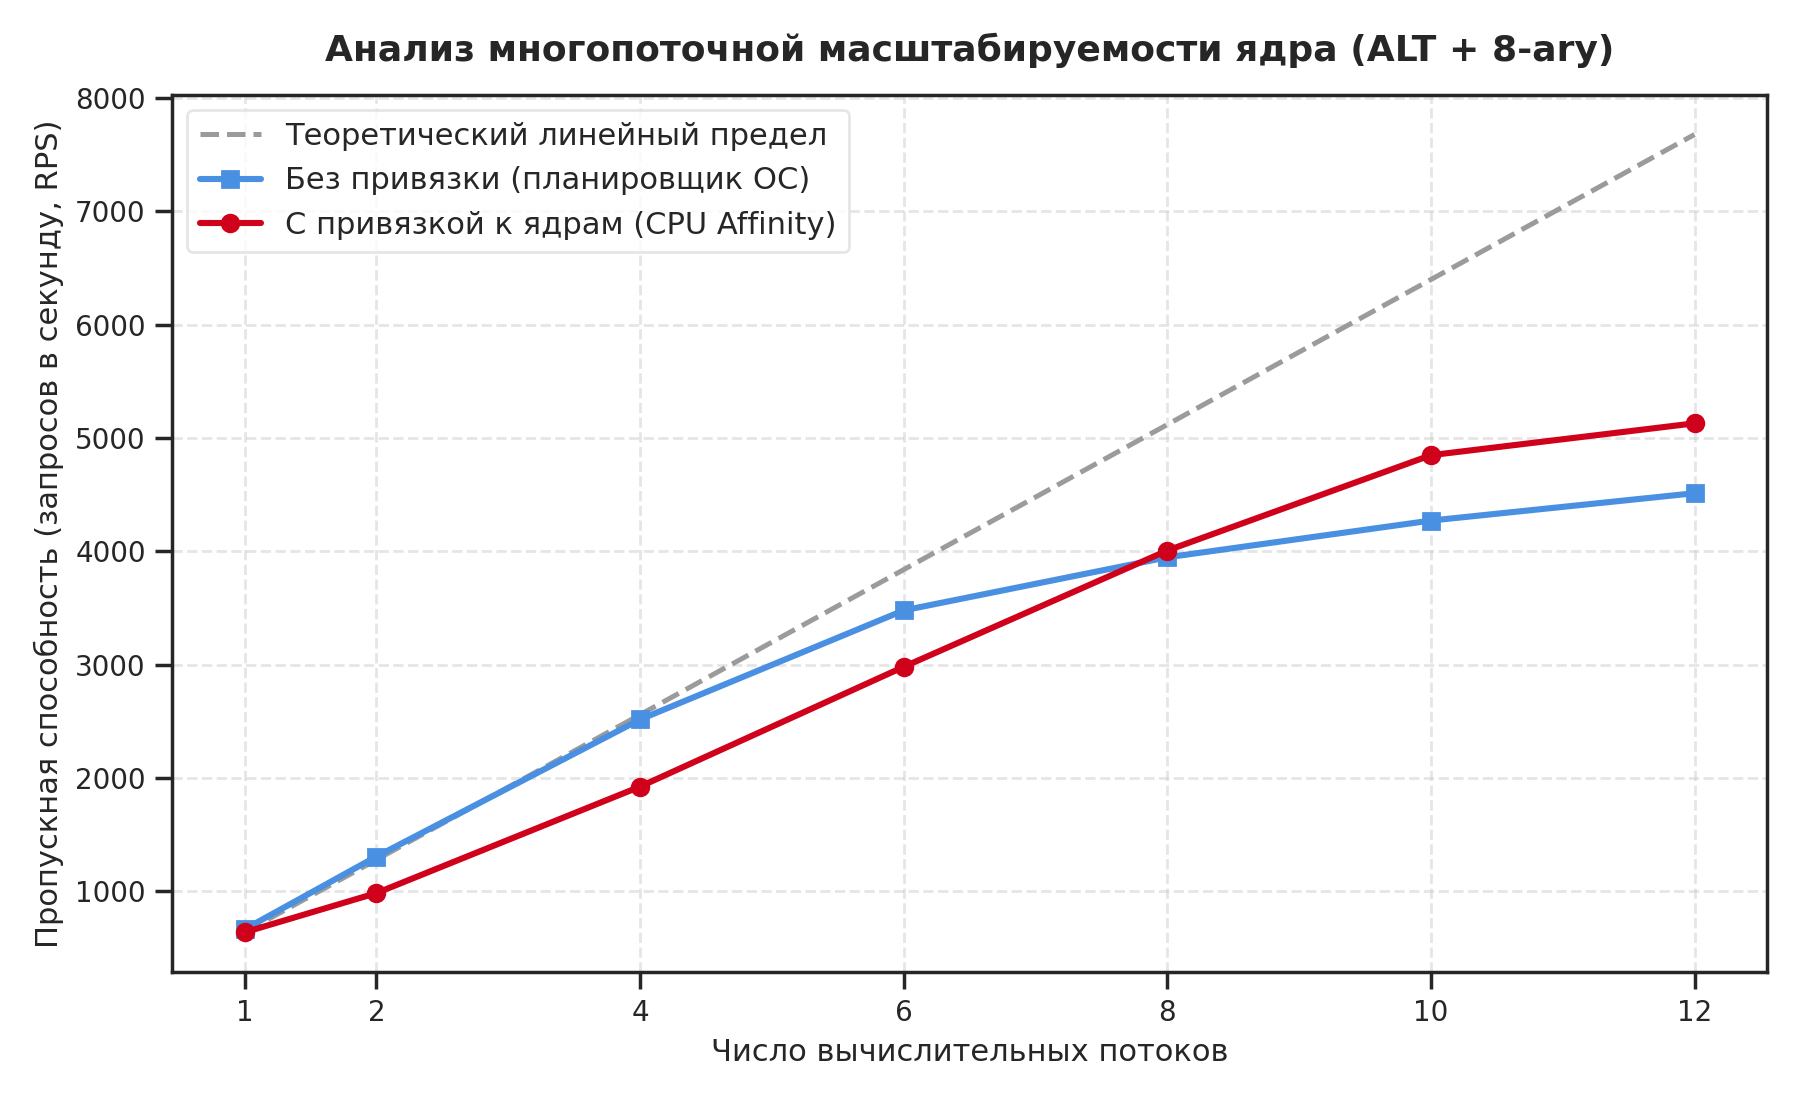
\includegraphics[width=0.85\linewidth,height=0.35\textheight,keepaspectratio]{assets/images/multithreading_scalability.png}
    \caption{Сравнение теоретического предела и фактической пропускной способности многопоточного ядра на базе алгоритма ALT и $8$-арной SoA-кучи}
    \label{fig:multithreading_scalability}
\end{figure}

Анализ графиков производительности позволяет выявить важный преломный момент масштабируемости. При числе потоков от $1$ до $6$ (что соответствует количеству физических ядер процессора AMD Ryzen $5$ 5600H) пропускная способность в обоих режимах растет практически линейно. В этой зоне планировщик операционной системы Linux эффективно распределяет нагрузку, а накладные расходы на миграцию потоков не оказывают заметного влияния. 

Преломный момент наступает при переходе за границу $6$ потоков. В диапазоне от $8$ до $12$ вычислительных потоков, когда задействуется технология одновременной мультипоточности (SMT) и потоки начинают делить аппаратные ресурсы физических ядер, стандартный планировщик операционной системы без привязки начинает хаотично мигрировать потоки между логическими ядрами. Это приводит к непрерывному сбросу L1 и L2 кэшей процессора и деградации производительности. В этой критической зоне жесткая аппаратная привязка вычислительных потоков к конкретным ядрам процессора выигрывает у планировщика операционной системы. При максимальной нагрузке в $12$ потоков режим с привязкой обеспечивает пропускную способность в $5130{,}63$ запросов в секунду (ускорение в $8{,}02$ раз относительно однопоточного режима), что на $13{,}6\%$ превосходит показатель без привязки ($4514{,}08$ запросов в секунду). Дальнейший рост сдерживается физической пропускной способностью шины оперативной памяти.

Необходимо отметить, что несмотря на использование безблокировочных очередей, на верхнем уровне диспетчеризации запросов в \texttt{StartRouterWorker} применяется барьерная синхронизация пакетов задач (\texttt{router\_pool\_.WaitForAll()}), соответствующая концепции Bulk-Synchronous Parallel (BSP). Данный барьер синхронизирует итерации распределения путей и вводит уязвимость к эффекту «длинного хвоста», когда один медленный запрос задерживает весь пакет. Однако в рамках разработанного ядра при QPS свыше $5000$ и низком среднем времени поиска пути ($3{,}93$~мс для ALT) данные накладные расходы остаются в пределах допустимого, не приводя к деградации общей пропускной способности симулятора.

Для обеспечения бесперебойного асинхронного обмена сообщениями между потоками симуляции, аналитики и маршрутизации программа сопоставляет стандартную блокирующую очередь на мьютексе, легковесный спинлок и высокопроизводительную безблокировочную очередь \cite{lock_free_queue, desrochers2015concurrentqueue} (библиотека \texttt{moodycamel::ConcurrentQueue}). Результаты сопоставления приведены на рис. \ref{fig:simulation_queue_comparison}.

\begin{figure}[htbp]
    \centering
    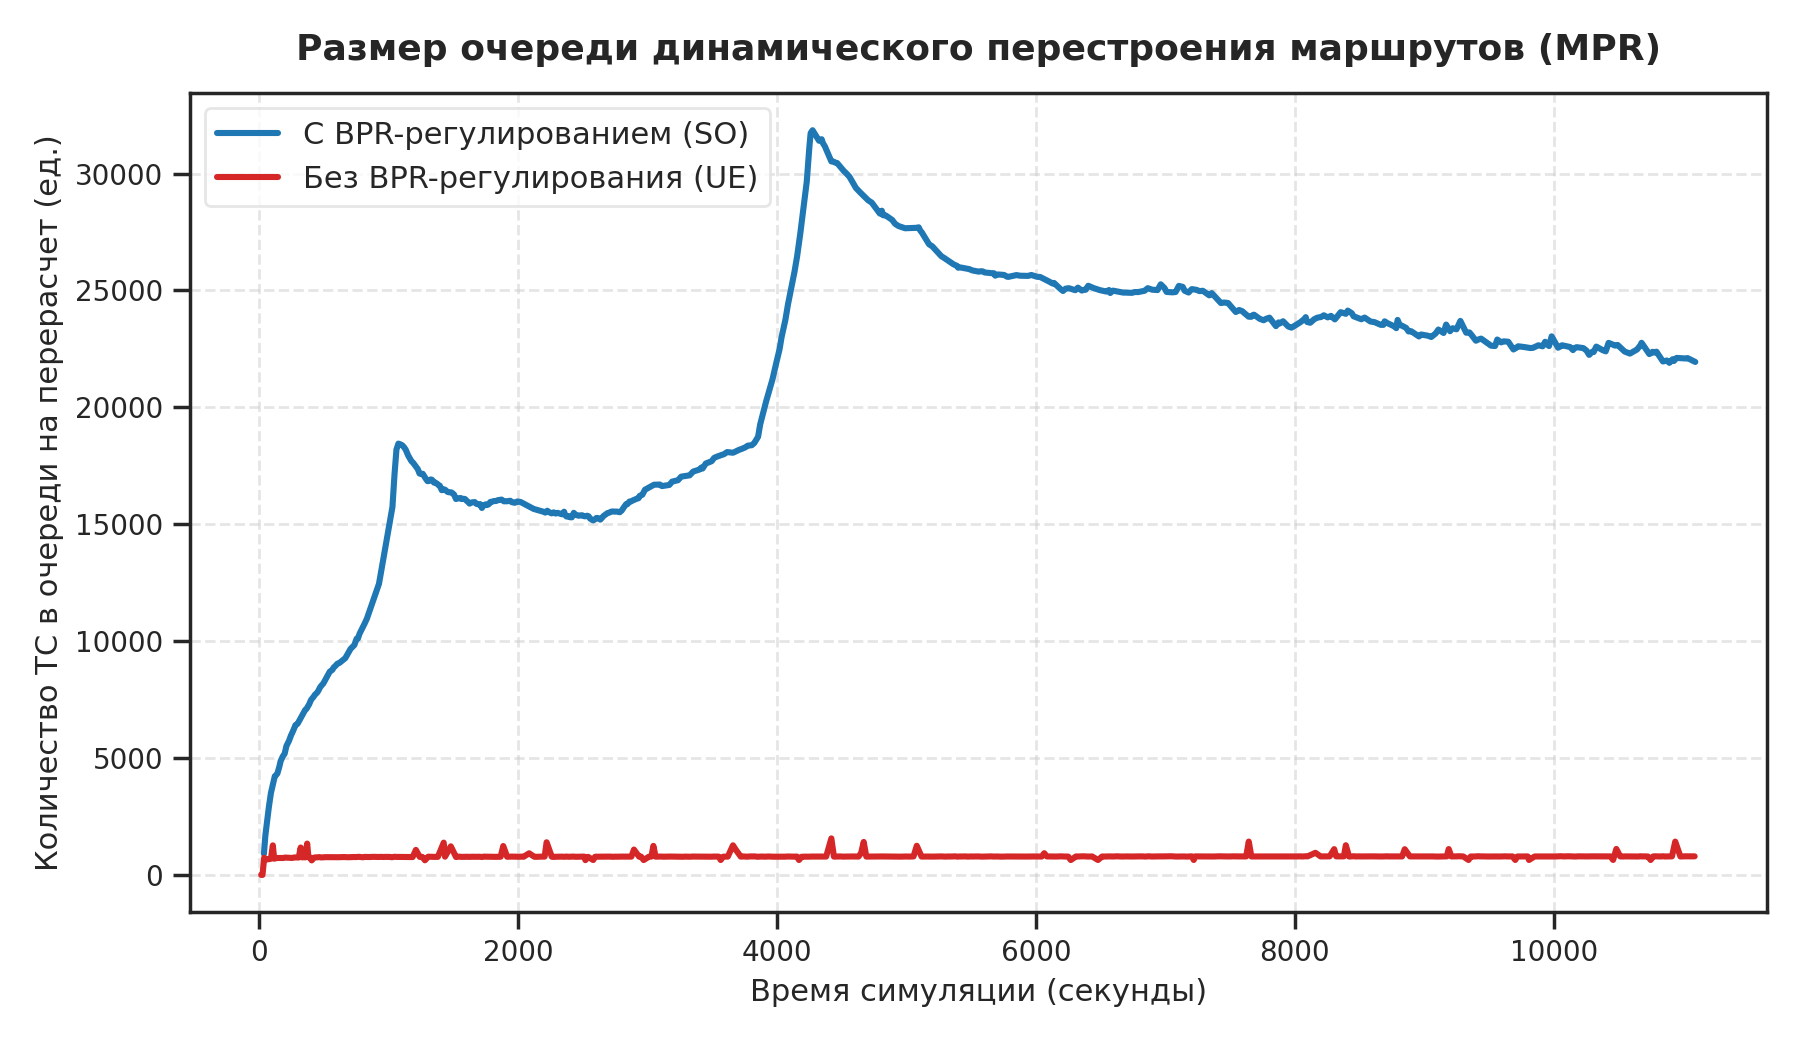
\includegraphics[width=0.85\linewidth,height=0.35\textheight,keepaspectratio]{assets/images/simulation_queue_comparison.png}
    \caption{Сравнение задержек асинхронного обмена сообщениями при высокой конкуренции потоков (мьютекс vs спинлок vs безблокировочная очередь)}
    \label{fig:simulation_queue_comparison}
\end{figure}

Блокирующая очередь на мьютексе вызывает лавинообразный рост задержек при увеличении числа конкурирующих потоков более $4$ из-за частого переключения контекста планировщиком операционной системы. Спинлок эффективен на малом числе потоков, но вызывает паразитный разогрев процессора при высокой конкуренции. Безблокировочная очередь обеспечивает стабильное время операции во всем диапазоне нагрузок, превосходя блокирующее стандартное решение в $8$--$10$ раз при $12$ конкурирующих потоках.
